\label{front_back_e000}

\begin{figure}[htbp]
\begin{center}
\begin{latexonly}
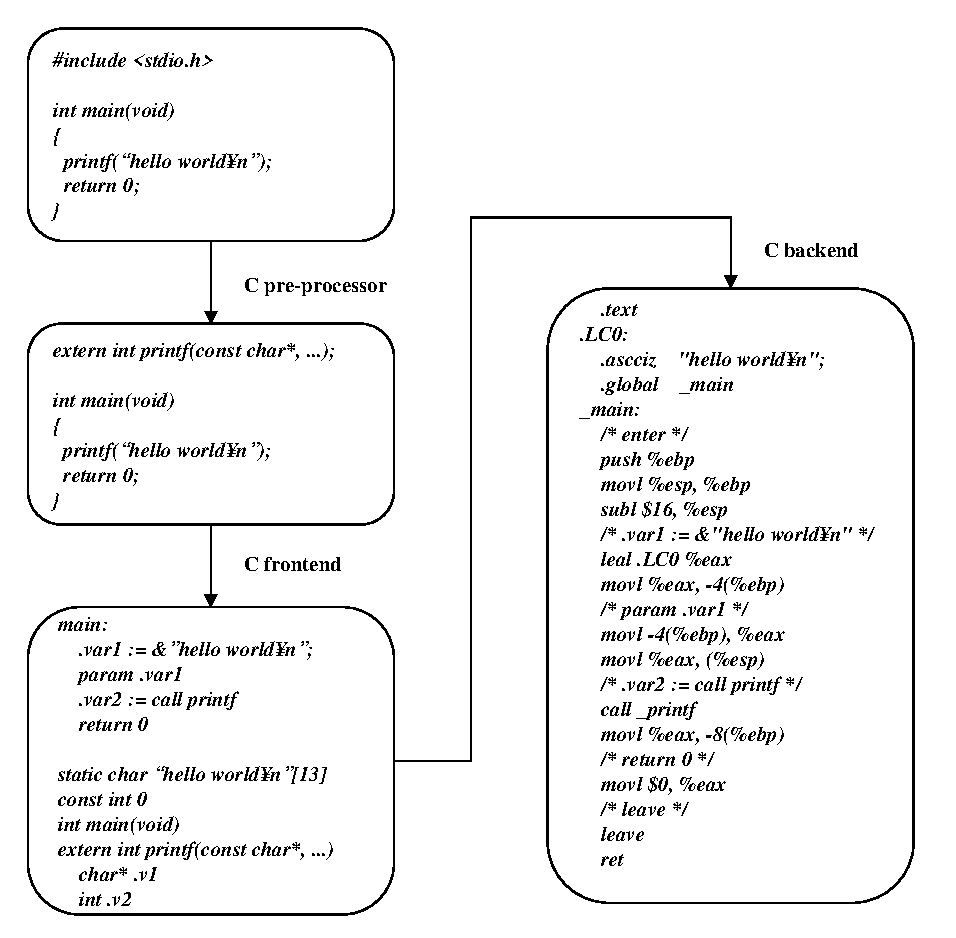
\includegraphics[width=1.2\linewidth,height=1.2\linewidth]{front_back_e.eps}
\end{latexonly}
\begin{htmlonly}
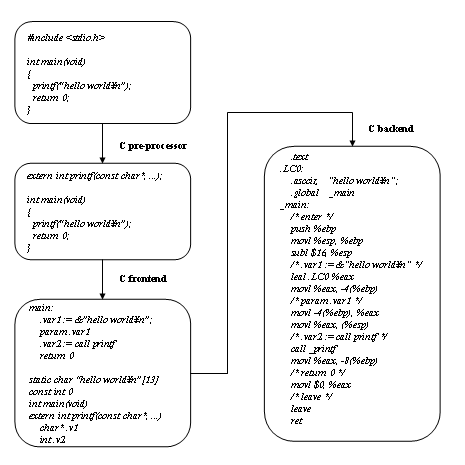
\includegraphics[width=1.2\linewidth,height=1.2\linewidth]{front_back_e.png}
\end{htmlonly}
\caption{frontend \& backend}
\label{front_back_e007}
\end{center}
\end{figure}
%% How to convert Power Point file to EPS file
%% http://keijisaito.info/arc/TeX/ve_ppfi_pdf.htm

To implement compilers for the various target processors, 
bibliography \cite{doragon} says that compilers should be devided into
 frontend \& backend.
Frontend is independent of target processsors
(depend on programming language), and backend is depend on
target processor. Figure \ref{front_back_e007} shows how they work
at programming language C `hello world'.

Frontend converts program to 3 address code and symbol table.
Backend converts outputs of frontend to target code(here, Windows/Intel code).

3 address code outputed by frontend is very simple for backend to
convert to target assembler code. Each operand of 3 address code
is an entry of symbol table, which contains name, type and storage class
or other infomation.

\begin{QandA}
Why is not Figure \ref{front_back_e007} target code optimized.

Answer : Mainly because backend which converts 3 address code to target code
doesn't optimize.

In compiler which constitute from frontend \& backend, each part
optimization makes optimized code.

This backend converts to about 3 instruction for an 3 address code.
Bibliography \cite{doragon} says that ``But if you convert 3 address code
 indiviually, you can only generate poor code'' at 9.1
(Sorry, but as you know, I just only read Japanese edition doragon book).
\end{QandA}

\begin{QandA}
\label{front_back_e003}
In figure \ref{front_back_e007} target code, address of string is saved
temporary variable. But generally, as a 3 address code,
\begin{verbatim}
param &y
\end{verbatim}
Is it allowable?

Answer : It should not be. We have to distinguish \tt{param y} and
\tt{param \&y}. And this 3 address code set including \tt{param \&y} is
redundant. On the other hand, at compile time, address of
variable, function or string literal is referenced as offset from
frame pointer or stack pointer, or label. This means target code
for \tt{param \&y} is better than obvious target code for
\begin{verbatim}
t0 := &y
...
param t0
\end{verbatim}
But it's possible to generate the same target code.
\end{QandA}

\begin{QandA}
In figure \ref{front_back_e007}, the return value of {\tt{printf}} 
is not used. It can be discarded?

Answer : It can be done at optimiezation phase.
\end{QandA}

